\documentclass{article}
\usepackage[frenchb]{babel}
\usepackage{amsfonts}
\usepackage{amsmath}
\usepackage[T1]{fontenc}
\usepackage[utf8]{inputenc}
\usepackage{amsthm}
\usepackage{graphicx}

\title{Géométrie de l'information et apprentissage distribué}
\author{Clément Dell'Aiera}
\date{}

\newtheorem{definition}{Def}
\newtheorem{thm}{Théorème}
\newtheorem{ex}{Exercice}
\newtheorem{lem}{Lemme}
\newtheorem{dem}{Preuve}
\newtheorem{prop}{Proposition}
\newtheorem{cor}{Corollaire}

\newcommand{\Z}{\mathbb Z}
\newcommand{\R}{\mathbb R}
\newcommand{\C}{\mathbb C}
\newcommand{\Hil}{\mathcal H}
\newcommand{\Mn}{\mathcal M _n (\mathbb C)}

\begin{document}
\maketitle

\begin{figure}[h]\centering
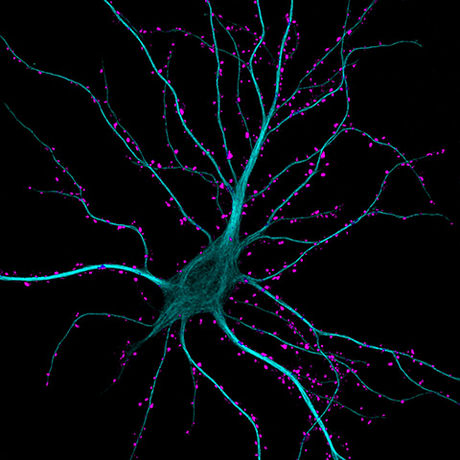
\includegraphics[scale=0.6]{Neurone.jpg}
\caption{Neurone grossi 63 fois, image de Kieran Boyle}
\label{fig:Neurone}
\end{figure}

\newpage
\tableofcontents

\newpage
%%%%%%%%%%%%%%%%%%%%%%%%%%%%%%%%%%%%%%%%%%%%%%%%%%%%%%%%%%%%%%%%%%%%%%%%%%%%%%%%%%%%%%%%%%%
\section{Point de vue géométrique en statistique}
%%%%

Parmi les premières méthodes d'apprentissage figurent celles utilisant des réseaux neuronaux. %Brève explication de ce qu'est un RN ?

Le but de ce travail est d'étudier ce réseau et d'appliquer les méthodes de géométrie de l'information pour peut-être mieux comprendre les raisons de leur efficacité.%Petit topo sur la géometrie de l'info ?

\subsection{Géométrie de l'information}

La géométrie de l'information propose d'utiliser les méthodes de la géométrie différentielle en statistique afin d'optimiser les algorithmes. Pour le lecteur apeuré par les gros mots mathématiques, qu'il se rassure : il n'est pas question ici d'étudier les propriétés géométriques fines des objets statistiques, mais plutôt d'appliquer des outils à peine plus sophistiqués que ceux d'un cours de calcul différentiel classique dans une optique d'optimisation.\\

 L'idée première est de donner une structure de variété différentielle au modèle statistique étudié : si $\mathcal S = \{p_\theta\}_\theta$ est notre honnête famille paramétrique de lois de probabilité, on peut voir $\theta \in \Theta$ comme une coordonnées, ou, pour parler le langage des géomètres, l'application : \[p_\theta \mapsto \theta\] fournit une carte locale. Petite remarque : cette application n'est définie que si le modèle est identifiable. On supposera d'ailleurs que le modèle a toutes les propriétés que l'on voudrait.\\

La deuxième étape est de donner une structure de variété riemannienne au modèle $\mathcal S$. Sans rentrer dans les détails, l'important est de savoir que l'on peut définir une métrique grâce à la log-vraisemblance $l$ du modèle par :
\[g_{ij} (\theta) = \mathbb E_\theta[\partial_i l(X,\theta) \partial_j l(X,\theta)]\]
En pratique, cela signifie que l'on peut mesurer des distances et des angles sur l'espace tangent à $\mathcal S$ : 
\[\forall w_1,w_2 \in T_\theta \mathcal S, \langle w_1 , w_2 \rangle = w_1^T G w_2\] où $G(\theta)=(g_{i,j}(\theta))_{ij}$.\\

Donnons un exemple important : celui des familles exponentielles. Le modèle est donné par :
\[\mathcal{E}xp(C,F,\psi) = \{p(x,\theta)=\exp[C(x)+\sum_{i=1}^n \theta^i F_i(x) -\psi(\theta)] \quad :\quad  \theta \in \R^n\}\]
où $F=(F_1,...,F_n)$ est une famille linéairement indépendante de fonctions $C^\infty$. Un simple calcul donne :
\[\partial_i \partial_j l(x,\theta) =-\partial_i \partial_j \psi(\theta)\]
Donc :
\[g_{ij}(\theta) =\mathbb E[\partial_i l(x,\theta)\partial_j l(x,\theta)]=-\mathbb E[\partial_i\partial_j l(x,\theta)]=\partial_i \partial_j \psi(\theta)\]
La matrice $G$ est donc la hessienne de $\psi$ et on a calculé la métrique riemannienne :
\[ds^2= \sum_{i,j} \partial_i \partial_j \psi \ dx^i dx^j\]

\subsection{Algorithme de descente de gradient naturel}

Amari décrit dans ses différents articles une méthode de descente de gradient adapté au cadre riemannien : on va corriger le pas par un facteur qui va se révéler être l'inverse de la matrice de Fisher. \textbf{idéeintuitive avec les ellipses, peut-être une illustration ?}\\

 On se donne une fonction de perte $L : \mathcal S \rightarrow \R$ que l'on évalue en $w$, et on veut minimiser $L(w+dw)$ où la norme $|dw|=\epsilon$ est fixée. 

\begin{thm}
La direction optimale de descente $dw^*$ est donnée par :
\[dw^*= -\hat{\nabla}L(w)=-G^{-1}(w) \nabla L(w)\]
\end{thm}

Donnons un sketch de preuve. Posons $dw= \epsilon a $, le problème de minimisation devient alors :
\[\min L(w+\epsilon a) \quad s.c. \quad |a|^2=\sum_{i,j} g_{ij}(w)a_i a_j=1\]

Mais $L(w+\epsilon a) - L(w)-\epsilon (\nabla L(w))^T a $ est un petit o de $\epsilon$ et minimiser $(\nabla L(w))^T a$ sous la contrainte $a^T G a = 1$ est simple avec les conditions de Lagrange qui donnent :
\[\frac{\partial}{\partial a_j}((\nabla L(w))^T a - \lambda a^T G a )=0\]
Finalement : $\nabla L(w) = 2\lambda Ga$ et donc 
\[a=\frac{1}{2\lambda}G^{-1}\nabla L(w)\] \qed\\

L'algorithme de pas d'apprentissae $\epsilon_n$ qui en découle est décrit par la formue de récurrence suivante :
\[w_{n+1}=w_n -\epsilon_n \hat{\nabla} L(w_n)\] 

%%%%%%%%%%%%%%%%%%%%%%%%%%%%%%%%%%%%%%%%%%%%%%%%%%%%%%%%%%%%%%%%%%%%%%%%%%%%%%%%%%%%%%%%%%%
\section{Réseau de neurones}

\subsection{Présentation}

Les réseaux de neurones ont initialement été développé comme des algorithmes, initialement dans le domaine de \textit{l'intelligence artificielle}, ce qui en fait naturellement une discipline du \textit{machine learning}. L'idée première était de s'inspirer du fonctionnement du cerveau humain pour créer des algorithmes adaptatifs. Bien que ce rôle fondateur de modèle pour le cerveau humain n'ai pas été un franc succès, les réseaux neuronaux ont donné des modèles statistiques intéressants. Ce changement d'interprétation est reflétée dans le nom de réseau de neurones \textit{artificiels} que certains auteurs utilisent désormais. \\

L'apprentissage est classiquement divisé en plusieurs domaines :
\begin{itemize}
\item apprentissage supervisé : apprendre à prévoir un output lorsque l'on donne un input, divisé en 2 catégories :
\begin{itemize}
\item régression 
\item classification
\end{itemize}
\item Non-supervisé : découvrir une bonne représentation de l'input.
\item Apprentissage par réenforcement : sélection des actions en maximisant le gain.\\
\end{itemize}
Les réseaux de neurones font partie de l'apprentissage supervisé : on se donne une liste d'exemple, le \textit{training set}, et l'on se sert de la différence entre la réponse attendue et la réponse donnée pour corriger l'algorithme.\\

Historiquement, on peut faire remonter l'origine des réseaux de neurones à McCulloch et Pitts en 1943 : ils proposent de modéliser formellement les neurones par des unités traitant un signal d'entrée, renvoyant en sortie un signal binaire correspondant à $1$ si le signal d'entrée dépasse un certain seuil, ce qu'ils nomment un \textit{binary threshold neurons} ou des unités de décisions.\\

Le perceptron constitue la première génération de réseaux neuronaux au sens où on l'entend aujourd'hui, popularisés par Fran Rosenblatt dans les années 60 et dont on trouvera un très bon exposé dans son livre \textit{Principles of Neurodynamics}.\\

Le lecteur pourra aussi trouver dans \textit{Perceptrons} de Minsky et Papert (1969) de quoi satisfaire sa curiosité. Ces deux auteurs sont à l'origine d'un résultat très négatif pour les perceptrons : le thèorème d'invariance sous l'action d'un groupe ("Group invariance theorem"), qui assure que les perceptrons ne peuvent pas apprendre des configurations invariantes sous l'action d'un groupe de transformations. Ce résultat est assez limitant puisqu'il empêche, par exemple, le perceptron d'apprendre des configarations de pixels qui sont invariantes par translations, typiquement ce qu'on aimerait lui faire faire. C'est là que les réseaux multicouches permettront de sauver la mise, comme nous le verrons.\\

Un réseau de neurones peut se formaliser de la façon suivante : plusieurs couches de neurones (que l'on imagine les unes superposées aux autres), chaque couche recevant des signaux de la couche précédentes. Chaque neurone $N_i$ est en fait un opérateur, qui agit sur les signaux d'entrés qu'il reçoit $y_j$ : il leur affecte chacun un poids $w_{ij}$ et ensuite une fonction, signal qu'il transmet à son tour :
\[y_i=f(b+\sum_{i\rightarrow j}w_{ij}y_j)=f(w^T.x)\]
où l'on prend $w$ le vecteur poids associé au neurone $N_i$.\\

Voici une liste non-exhaustive de différents réseaux de neurones, que l'on présente en fonction de leur fonction de réponse :
\begin{itemize}
\item binaire : $y=1_{b+w^Tx>0}$
\item linéaire : $y=b+w^Tx$
\item linéaire rectifié : $y=max(0,b+w^Tx)$
\item sigmoïde : $y=\frac{1}{1+e^{-z}}$
\item binaire stochastique :$\mathbb P(s=1)=\frac{1}{1+e^{-z}}$ L'output est traité comme le paramètre de Poisson.\\
\end{itemize}

Ainsi que plusieurs types d'architectures que l'on peut leur imposer, c'est-à-dire comment les neurones sont reliés entre eux :
\begin{itemize}
\item Une couche ou plusieurs (deep neural networks)
\item Récurrents : des cycles sont possibles.
\item Complets.
\item Toute structure imagnable sur un graphe ! En fait, le modélisateur n'est pas obligé d'adopter une strucutre en couches.\\
\end{itemize}

%%à réaccorder correctement
Ces réseux peuvent se reformuler en termes de modèles statistiques, comme Herbert K.H.Lee l'expose dans \textit{Bayesian Non Parametrics via Neural Networks}. Rappelons qu'un réseau est composé de plusieurs couches : la couche d'entrée, les couches cachées et la couche de sortie. Chaque noeud du réseau applique une fonction $\psi$, en général une sigmoïde, à une combinaison linéaire des signaux d'entrée. Si $y$ est le signal de sortie, $x$ l'entrée, le modèle statistique que représente le réseau à $m$ couches cachées prend souvent la forme :

\[y=\beta_0 \sum_{i=1}^m \beta_i\psi(w_i^T x_i) + \eta_i\]
\[\eta_i \sim \mathcal N(0,\sigma^2)\]

Cet équation montre qu'un réseau neuronal peut s'interpréter comme un modèle de régression non paramétrique sur une base donnée. Par exemple, si 
\[\psi(x)=\frac{1}{1+\exp(-x)}\]
est la fonction logistique, on sait que l'espace engendré par les translatés-échelonnés de cette fonction est tout l'espace des fonctions de carré intégrable.

%Un exemple simple : 2 couches de  neurones.
%\begin{itemize} \item Top $=$ formes connues. \item Bottom $=$intensité des pixels.\end{itemize} Chaque pixel peut voter (pour plusieurs formes) s'il est colorié. \\

Détaillons un peu différents modèles simples de RN.

 \subsection{Neurones binaires et algorithme du "perceptron convergence procedure"}
Ces neurones ont une fonction deréponse de type indicatrice :
\[y=1_{\{w^Tx\geq 0\}}\]

Voici comment entraîner les neurones binaires comme classifiants :\\

\fbox{\begin{minipage}{0.9\textwidth}
\begin{enumerate}
\item Incorporer une composante $1$ en plus au vecteur input, pour incorporer le biais dans les poids.
\item Choisir un exemple d'entraînement. La procédure de choisx doit assurer que tous les exemples seront choisis.
\item Si l'output est correct, ne pas changer les poids. Sinon soustraire l'input du vecteur des poids.
\end{enumerate}
\end{minipage}}\\
\\

On peut interpréter géométriquement cette procédure.\\

L'ensemble des poids est vu comme un $\R$-espace vectoriel de dimension le nombre de poids. Un input définit un hyperplan (son orthogonal), et un vecteur poids donne la bonne réponse par rapport à cet input ssi il est du "bon côté" du plan. Si on a deux inputs, le sous-ensemble des bons poids (qui répondent correctement aux deux inputs) forment alors un cône. On remarque que les bons poids forment un ensemble convexe : le problème est convexe.\\

Preuve :\\%la faire vraiment
On suppose qu'il existe un vecteur $w^*\in C$ qui donne la bonne réponse à tous les exemples.\\
\[|w_{n+1}-w*|^2=|w_n-x|^2=|w_{n+1}|^2+|x|^2+2\langle w_n,x\rangle+|w^*|^2+2\langle w^*,w_n-x\rangle \leq |x|^2\]

\subsection{Neurones linéaires ou filtres linéaires}
On appelle neurones linéaires des neurones dont la focntion de réponse est linéaire :
\[y=w^Tx\]

Ici l'algorithme, plutôt que d'approcher de mieux en mieux le poids idéal, va optimiser la distance entre l'ouput et la cible, ce qui est une différence notable par rapport au cas précédent. La procédure des neurones binaires (perceptron) ne peut pas se généraliser à plusieurs couches et nous prévenons le lecteur : leur nom de "perceptron multicouches" utilisé à propos des neurones linéaires est un faux ami ! \\

Voici l'algorithme :\\

\fbox{\begin{minipage}{0.9\textwidth}
Choisir un pas d'apprentissage $\epsilon$.
\begin{enumerate}
\item On entraîne en donnant la cible $t$.
\item Actualiser les poids selon : \[\Delta w_i = \epsilon x_i(t-y)\]
\end{enumerate}
\end{minipage}}\\
\\

On comprend que cet algorithme n'est rien d'autre qu'une descente de gradient. En effet, si on dérive l'erreur quadratique : \[E=\frac{1}{2}\sum_{n\in training}(t^n-y^n)^2\]
on obtient : $\frac{\partial E}{\partial w_j}=-\sum x_i^n(t^n-y^n)$. Cette règle d'actualisation des poids (\textit{batch delta-rule}) modifie les poids proportionnelement à cette dérivée afin de se rapporcher du minimum de la surface d'erreur :
\[\Delta w_i =-\epsilon \frac{\partial E}{\partial w_j}\]


\subsubsection{La surface d'erreur du neurone linéaire}
On se place dans l'espace des poids, augmenté d'une dimension pour l'erreur. On s'intéresse donc au graphe de l'erreur :

\[\mathcal S = \{(w_1,..,w_n,E)\}\]

Dans le cas d'un RN linéaire avec erreur quadratique, c'est un paraboloïde elliptique. L'algorithme précédent effectue une descente le long de ce paraboloïde, perpendiculairement aux lignes de niveau (qui sont des ellipses). Cela explique que l'apprentissage puisse être très lent : si l'ellipse est très aplatie, le gradient peu pointer dans une direction très peu colinéaire au minimum recherché. ( d'où la correction avec le gradient riemanien)

\newpage
\begin{figure}[!h]\centering
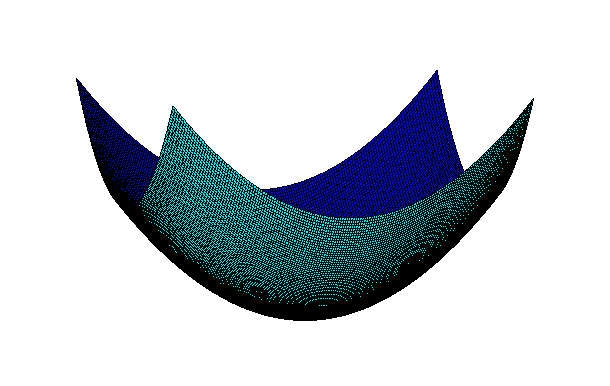
\includegraphics[scale=0.5]{Surfaceerreur.png}
\caption{La forme typique d'une surface d'erreur quadratique.}
\label{fig:Surface}
\end{figure}

\begin{figure}[!h]\centering
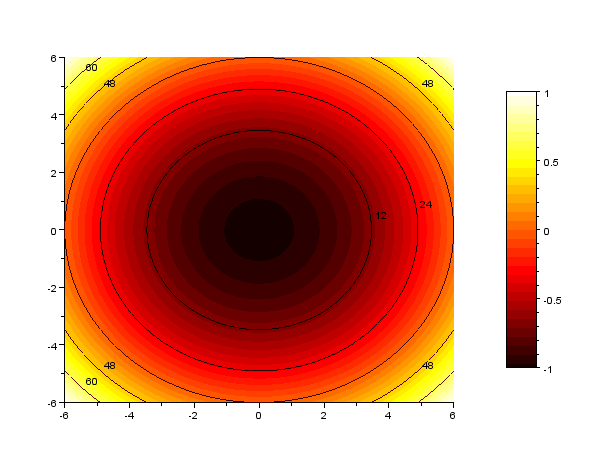
\includegraphics[scale=0.5]{level.png}
\caption{Les lignes de niveau d'une surface d'erreur quadratique sont bien des ellipses. }
\label{fig:level}
\end{figure}

\newpage
\subsection{Neurones logistiques}

On va généraliser la procédure précédente aux réseau de neurones logistiques, ceux qui ont une fonction de réponse du type : 
\[z=b+w^Tx\]
\[y=\frac{1}{1+e^{-z}}\]
On remarque que l'image de la fonction logistique est l'intervalle $(0;1)$, ce qui nous permettra d'interpréter sa valeur comme la probabilité de l'output sachant l'input, dans le cas de réseaux de neurones stochastiques. 
\[\frac{\partial y}{\partial w_i}=x_i y(1-y)\]
\[\frac{\partial E}{\partial w_j}=-\sum_{n}x_i^n(1-y^n)y^n(t^n-y^n)\]

\subsection{Algorithme de rétropropagation}

Maintenant que l'on sait modifier les poids pour une seule couche, on va donner un moyen de modifier les poids dans le cas de couches cachées. Cette généralisation n'est pas innocente : les réseaux sans couche cachée ne sont pas très adaptables, au sens où leur modélisation est beaucoup plus limitée que celle des réseaux multicouches. L'idée de la rétropropagation est de remonter les dérivées des erreurs par rapport au output récursivement à travers les couches cachées, de la couche des ouptu à celle des input. On suppose bien sûr que l'erreur est dérivable, rendant cet algorithme inutile pour un réseau binaire par exemple.\\

Soit donc un neurone $N_j$ situé dans une couche cachée. Il reçoit un input total 
\[z_j=\sum_{i\rightarrow j} w_{ij}y_i.\]
On cherche alors à calculer l'erreur $\frac{\partial E}{\partial y_i}$ pour tous les neurones qui lui sont connectés dans la couche précédente, \textit{ie} les neurones $N_i$ tels que $i\rightarrow j$. Mais une simple application de la règle de la chaîne donne une expression simple pour ce terme :

\[\frac{\partial E}{\partial z_j}=\frac{\partial y_j}{\partial z_j}\frac{\partial E}{\partial y_j}=y_j(1-y_j)\frac{\partial E}{\partial y_j}\]
\[\frac{\partial E}{\partial y_i}=\sum_j\frac{\partial z_j}{\partial y_i}\frac{\partial E}{\partial z_j}=\sum_j w_{ij}\frac{\partial E}{\partial z_j}\]
Donc :\\

\fbox{\begin{minipage}[c]{0.45\textwidth}
\[\frac{\partial E}{\partial y_i}=\sum_j w_{ij}y_j(1-y_j)\frac{\partial E}{\partial y_j}\]
\end{minipage}}\\
\\
On peut alors caculer la variation de l'erreur en fonction d'une variation des poids :
\[\frac{\partial E}{\partial w_{ij}}=\frac{\partial z_j}{\partial w_{ij}}\frac{\partial E}{\partial z_j}=y_i\frac{\partial E}{\partial z_j}.\]

Bien que cette procédure nous guide pour adapter les poids, plusieurs questions se posent en pratique, par exemple : à quelle fréquence doit on mettre à jour nos poids ? Comment choisir la vitesse d'apprentissage ? On peut adapter les poids à chaque exemple (\textit{online}), après tout le stock d'exemple (\textit{full batch learning}), ou bien encore après un petit nombre (\textit{mini batch}).\\

%%%%%%%%%%%%%%%%%%%%%%%%%%%%%%%%%%%%%%%%%%%%%%%%%%%%%%%%
\subsection{}
Softmax : forcer les outputs à former une probabilité
Problème de l'erreur quadratique : mauvais avec une fonction logistique , les dérivées tendent à "plateau out" lorsque l'output $y$ ets proche de $0$ ou $1$ : 
\[\frac{dE}{dz}=(t-y)y(1-y)\]
Une erreur plus convenable est la cross entropy function :
\[E=-t\log(y)-(1-t)\log(1-y)\] 
car alors \[\frac{dE}{dz}=y-t\]
Pour un groupe de neurones $N_i$ qui recoivent en entrée $z_i$ appelée \textit{logit}, l'output est donné par 
\[y_i=\frac{e^{z_i}}{\sum_{j\in group} e^{z_j}}\]
\[\frac{dy_i}{dz_i}=y_i(1-y_i)\]
Corss entropy : la bonne fonction de coût \[C=-\sum_j t_j \log(y_j)\quad t_j \ \text{target value}\]

\subsection{Point de vue géométrique}

Nous présentons dans cette section les idées de différents articles d'Amari, ainsi que de son livre \textit{Methods of information Geometry}.\\

Comme nous l'avons remarqué, les réseaux de neurones peuvent s'interpréter comme un modèle statistique à réponse non linéaire : $y=f(x,w)$, et en supposant que les données suivent la densité $q(x)$ et qu'on a la densité conditionnelle $p(y|x,w)$, l'ensemble des données $(x,y)$ suivent la loi :

\[q(x)p(y|x,w)\]

Les modèles de perceptrons que nous présenterons ensuite sont considérés pa Amari comme des points d'une variété qu'il appelle \textit{Neuromanifold}, où les coordonnées sont les $w$ et la métrique est donnée par l'information de Fisher.\\

Un autre exemple fortement lié aux réseaux de neurones est celui de la \textbf{machine de Boltzmann}, qui est un réseau totalement connecté de $n$ neurones stochastiques. Chacun des neurones $N_i$ possède un état $x_i$ qui est $0$ ou $1$, qu'il communique en \textit{output} aux autres neurones. \\
Chaque neurone calcule la quantité
\[u_i=\sum_{j \neq i} w_{ij}x_j-h_i\]
en fonction des signaux qu'il reçoit. Le poids $w_{ij}$, appelé poids de la connexion synaptique, mesure l'influence du neurone $N_j$ sur le neurone $N_i$, et $h_i$ est appelé le seuil de $N_i$. On suppsoe que la matrice des poids $W= [w_{ij}]$ est symmetrique à diagonale nulle.\\
A chaque étape, chaque neurone $N_i$ détermine s'il sera dans l'état excité $1$ ou dans l'état de repos $0$ selon la probabilité :

\[\mathbb P(x_i=1)=\frac{e^{u_i}}{1+e^{u_i}}\]

L'état de la machine de Boltzmann est représenté par le vecteur $x=(x_1,...,x_n)$, qui suit une chaîne de Markov sur l'espace de tous les états possibles, espaces à $2^n$ points. Cet chaîne admet comme loi stationnaire :
\[p^{W,h}(x)=\frac{1}{Z}\exp\{-E(x)\}\]
\[\text{avec} \quad E(x)=-\frac{1}{2}x^TWx +h^Tx\]
\[\text{et} \quad Z=\sum_x \exp\{-E(x)\}\]

On peut prendre le point de vue géométrique en se représentant la machine de Boltzmann comme une système qui se comporte selon la loi stationnaire $p^{W,h}(x)$, donc comme un point de coordonnées $(W,h)$ dans la variété de toutes les machines de Boltzmann. ( Encore un exemple de famille exponentielle. )

\subsection{Multilayer Neural Network}

On se donne un réseau de neurones spécifié par un paramètres $w\in \R^n$, qui représente les poids modifiables des connexions entre les synapses. En entrée du réseau, le signal $x$, qui suit une loi de probabilité inconnue $q(x)$, est traité, et le réseau calcule une sortie $f(x,w)$. \\

Le but est d'entraîner les neurones : on est en apprentissage supervisé. Lorsque l'on donne l'entrée $x$ au réseau,on peut donc lui spécifier quelle sortie $y$ lui correspond. La discussion qui suit permettra de comprendre comment nous pouvons élaborer un algorithme qui, par itération, améliore les poids jusqu'à atteindre un poids possiblement optimal $w^*$.\\

Soit $L$ une fonction de perte, typiquement : 
\[L(x,y,w)  = ||y-f(x,w)||^2.\] 
En considérant un modèle statistique où le but est une version bruité du signal de sortie, avec un bruit normal centré, ie :
\[y=f(x,w)+\eta\]
\[\text{avec} \quad \eta \sim \mathcal N (0,I_n)\]
la densité du couple $(x,y)$ prend la forme :
\[cq(x)\exp\{-\frac{1}{2}||y-f(x,w)||^2\}.\]

Face à une série d'exemples $(x_1,y_1),...,(x_N,y_N)$, l'algorithme naturel de descente est donné par :
\[w_{n+1}=w_n - \epsilon_n \nabla l(x_n,y_n,w_n), \]
où $l$ est le $\log$ de la densité du couple $(x,y)$, et $\epsilon_n$ est le pas d'apprentissage. Cet algorithme nous fait nous déplacer sur l'espace des réseau de neurones paramétrés pas $w$. Dans Amari\textit{1985}, on peut donner une structure de variété riemannienne à cet espace, structure dont la métrique est donnée par :
\[g_{ij}(w)=\mathbb E[\partial_i p(x,y,w)\partial_j p(x,y,w)].\]

\subsection{Cas du perceptron}

On peut obtenir une forme explicite pour le percptron multicouche.
Ici, la fonction signal est donnée par : \[f(u)=\frac{1-e^{-u}}{1+e^{-u}}\], et $y=f(w.x)+\eta,\quad \eta \sim \mathcal N (0, \sigma^2)$.\\

La densité conditionnelle de $y$ sachant $x$ est alors :
\[p(y|x,w) = \frac{1}{\sqrt{2\pi}\sigma}\exp\{-\frac{1}{2\sigma2}||y-f(x,w)||^2\},\]
ce qui, combiné à l'hypothèse $q(x)$ gaussienne, donne une densité jointe :

\[p(x,y,w) = q(x)p(y|x,w) \]

Le théorème suivant, dont la preuve se trouve dans  \textit{Natural Gradient worksefficiently in learning}, donne explicitement la forme de la métrique de Fisher dans le cas du perceptron multicouches, sous nos hypothèses.

\begin{thm}{(Amari)}
La métrique de Fisher vaut : 

\[G(w)=|w|^2 c_1(w)I_n + (c_2(w)-c_1(w))w\otimes w\]
où :
\[c_1(w)=\frac{1}{4\sqrt{2\pi}\sigma^2|w|^2}\int (f^2(wt)-1)^2\exp(-\frac{1}{2}t^2)dt\]
\[c_2(w)=\frac{1}{4\sqrt{2\pi}\sigma^2|w|^2}\int (f^2(wt)-1)^2t^2\exp(-\frac{1}{2}t^2)dt\]

La matrice inverse est : 
\[G^{-1}(w)=\frac{1}{|w|^2 c_1(w)}I_n+\frac{1}{|w|^4}(\frac{1}{c_2(w)}-\frac{1}{c_1(w)})w\otimes w\]
\end{thm}
 
Nous pouvons alors donner une formule explicite pour l'algorithme de gradient naturel :
\[w_{n+1}=w_n + \epsilon_n(y_n-f(w_n.x_n))f'(w_n.x_n)
	\{ \frac{1}{|w_n|^2c_1(w_n)}x_n+\frac{1}{|w_n|^4}( \frac{1}{c_2(w)}-\frac{1}{c_1(w)}) w_n.x_n w_n\}\]

En guise de remarque finale pour cette partie, mentionnons que cette méthode se généralise facilement ( bien qu'avec plus de calculs ) au cas d'un perceptron multicouche à sortie linéaire, possédant $m$ couches. 
La relation \textit{input-output} s'écrit ici :
\[y=\sum_{i=1}^m v_i f(w_i.x)+\eta\]
\[\eta \sim \mathcal N(0,I_n)\]

Le calcul de $G^{-1}$ est plus facile que dans le cas classique ( comparez l'inversion d'une matrice $(n+1)\times m$ à celle d'une matrice $2 \times (m+1)$ ), et Amari et G. Yang ont effectué des études sur cette méthode : elle pourrait éviter l'effet plateau que les méthodes classiques peinent tant à eviter.

\section{Application à la reconnaissance de caractères manuscrits}

\subsection{Rappel sur les ondelettes}
Les ondelettes forment des bases hilbertiennes de $L^2(\R)$ en partant d'une fonction $\phi$, appelée fonction mère, que l'on translate-échelonne ensuite : 
\[\{2^{j/2}\phi(2^j . -k)\}_{k\in \Z, j \in \Z}.\]
Par exemple la fonction mère $\phi(u)=1_{0<u<\frac{1}{2}}-1_{\frac{1}{2}<u<1}$ donne la base de Haar, très utilisée en traitement d'image. Voici quelques une de ces fonctions :
\begin{figure}[h]\centering
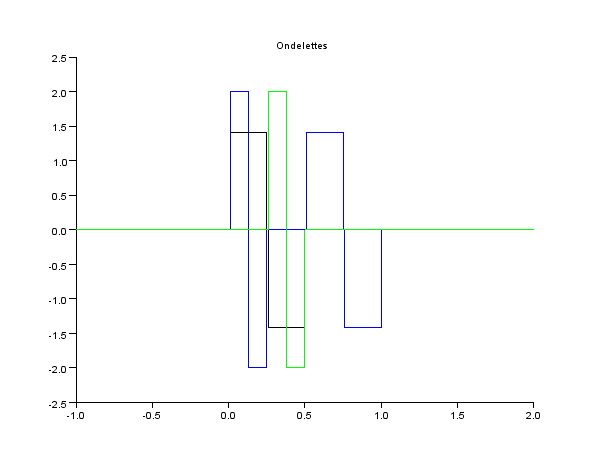
\includegraphics[scale=0.4]{Ondelettes.png}
\caption{Ondelettes tracées avec Scilab}
\label{fig:Ondelettes}
\end{figure}

\subsection{Description de l'algorithme}
On entraîne le réseau de neurones avec des images de lettres manuscrites et de la lettre correspondante. Les images sont représentées par un vecteur $N$ dimensionnel, dont les coordonnées sont les $N$ premiers coefficients sur la base d'ondelette.

\section{Deep Learning vs Support Vector Machine}

Première Deep Learning architecture : Neocognitron.\\
Idée : entraîner une couche à la foisen la tratiant comme une machine de Boltzmann restreinte (RBM), et ensuite appliquer un algorithme de Backpropagation.\\
Rôle de Yan Lecun : première utilisation de l'algorithme de Backpropagation. Disponible depuis les années 70s,cet algorithme était considéré comme trop lent en pratique : problème du vanishing gradient.\\
\textbf{Algo $em$ et $EM$ ?}

%%%%%%%%%%%%%%%%%%%%%%%%%%%%%%%%%%%%%%%%%%%%%%%%%%%%%%%%%%%%%%%%%%%%%%%%%%%%%%%%%%%%%%%%%%%
\section{Appendice}

\subsection{Géométrie différentielle}




\end{document} 



































